%!TEX root = project.tex

\chapter{Methodology}

For the project we used the waterfall methodology. We started by mapping out the requirements for the project. Then we designed how the UI would be implemented, how the user should be able to add an account on the system.  We used GitHub for source control of the program, we also used overleaf for collaboration with the dissertation.

We had regular meetings as a group and also with the group supervisor to discuss issues we were facing with the project and to make any changes that needed to be made.

\section{Requirements}

We mapped out the requirements of our project:
\begin{itemize}
\item We would need a server or some form of central point that connects the users to any back-end that we would require to run the game.
\item We decided the system required a login system that would allow a user to create an account or login to an existing one.
\item We then would need a system that allowed players to connect to other users.
\item We would need a lobby systems where players can wait for a game to start or wait for other players to join the game.
\item Once the game has ended we would need a system that could keep track of the players games and achievements such as a scoreboard system.
\item The separate systems speak to the client and do not need to send data to each other, this will allow the system to be interchangeable.
\item Element of the system should be capable of being replaced by another system, without replacing other parts of the system. For example, if we decided to change the database or language for the scoreboard system, we should be able to do so without having to change any part of the login system, the match making system and minimal changes to the game itself, if any.
\end{itemize}


The game Itself:
\begin{itemize}
\item Must have a procedural track to allow for non repetitive play.
\item Different versions of the game should connect to any instance and should not need to specify whether they can play with desktop or virtual reality headset users.
\item Desktop platforms must be able to see head and hand movement from the head mount display players.
\item Players must start in specified positions and must not have to enter any input for this to occur.
\item The Races must have a start and end point.
\end{itemize}

\newpage
\section{Design Stage}

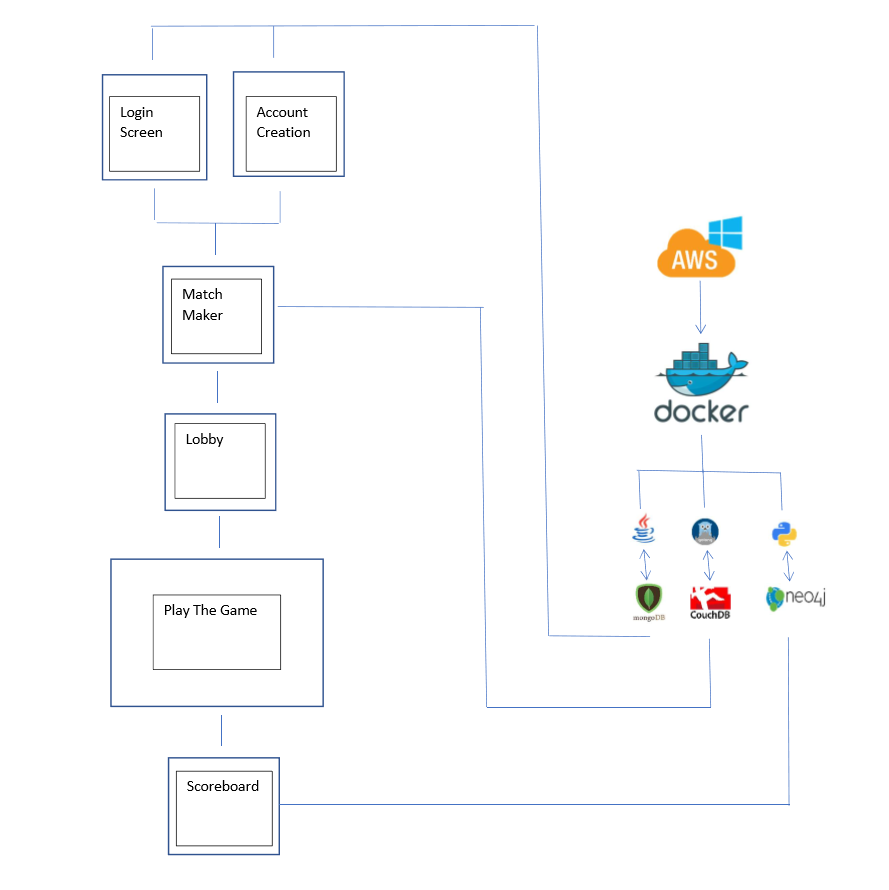
\includegraphics[width=1\columnwidth]{img/Overview.PNG}
\subsection {Overview}
The design stage is a critical and vital part of a software development project. Without first setting out goals and deliverance's, a project can quickly lose it way. Design and modelling have been used in various projects dating back to the Ancient Egyptians and Romans and has been used many civilization's since. This process is widely used in science and engineering to give a high-level view of the system.
\newline

The first stage is to create a design document and a model of the intended project. This document is a detailed layout of the system used to give an overall guide to the architecture of the project.
It should include attributes and relationships between data and their structures along with architectural, interface and procedural designs.
\newline

The next stage is to design a model of the project. This model is then used to obtain a better understanding of the system and is referenced to help understand the flow of data the various steps that take place throughout the project. 
\cite {36160220110101}
\bibliographystyle{plain}
\newline

The next stage of design is the analysis stage. This part of the process is about analyzing the performance of the various stages of the software and its requirement and limitations. This is a vital part of the process and extremely relevant to our project as there was many different technologies and programming languages used. With these factors researched and discussed, we began the task of designing our project.
\newline

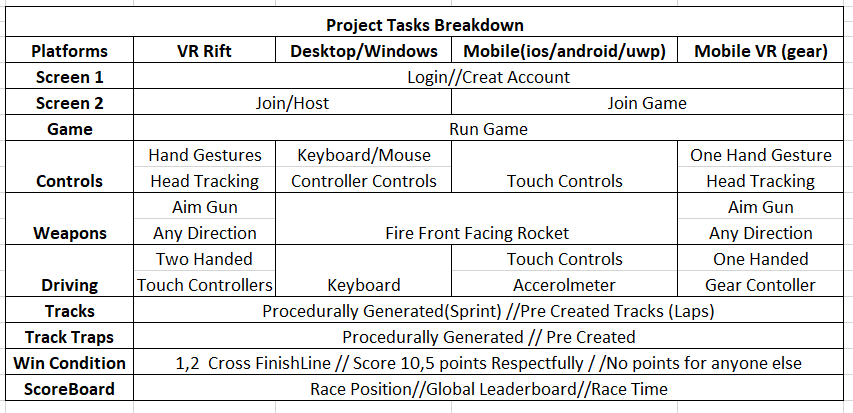
\includegraphics[width=1\columnwidth]{img/breakdown.PNG}

\subsection {The Game}
During the design stage, we had to map out the system and decide on which elements were needed and how they could be implemented. From the very start we knew that the game itself must be implemented in either Unity with C\# or using the Unreal 4 engine with C ++. Our knowledge and experience of the unreal engine and with any of the C language is very limited, where as we already have a working knowledge of unity and C\#. So we went with Unity. Using any form of third gaming engine would not be practical as the libraries for the virtual reality devices have been focused on these two implementations.\newline

\subsection {System Back-end}
We then needed to consider the back-end of the system and which platform were available. Firstly we could have used a physical computer that we personally owned and set it up as a running server. This would not have been a bad idea as we already own personal computers that could have effectively done this. Other options included using cloud based servers such as Amazon Web Services(AWS) or Google cloud. We had setup some instances of google cloud, we even ran them and began launching some of the programs on the system. From prior experiences, we had encountered situations were we had been charged by google cloud for use of such cloud instances and had found(AWS) to be a much cheaper rate. We also had some prior experience with AWS and opening firewall rules for this service, as we are using sockets, this was certainly going to be needed.\newline

\subsection {Login system}\newline
Development of the login system started with creating two java programs that used sockets to make a connection to one another. A socket is one endpoint of two-way communication between two programs running on a network with a corresponding socket on the other end. Each socket is bound to a port number that the TCP layer can identify that allows data to be sent back and forth between the two programs.\newline

Before development went any further a decision was made to use MongoDB as our database for the user login. The installation of MongoDB involved logging into the AWS virtual machine we are using for our project. For this project we decided to use the free version of MongoDB known as the community version using the current stable release (4.0.3) (MSI).\newline

Once the two java programs were up and running a number of basic tests were performed to verify the programs were working correctly by sending and receiving basic information across the connection. The next step was to take the existing program and use it to receive a connection from the unity game scene in the user login details page. This required making major modifications to the existing java programs.\newline

For this project our database is called usersdb and our collection is called users. Once the database was set up and installed we got to work on the two java programs. After the java programs were up and running we performed a number of basic tests to verify the programs were working correctly by sending and receiving basic information across the connection. The next step was to take the existing program and use it to receive a connection from the unity game scene in the user login details page. This required making major modifications to the existing java programs.\newline

The modifications involved creating several new java programs to receive a connection from the server and connect to the database. Then we created a user object in the java program that consisted of a username and password. We created an interface called database connection that contains the methods to add users, find users and verify passwords.\newline

This involved making a connection using a C\# login script in visual studio, through sockets, on port numbers 5000 and 5001. The login details page in the unity project required a username and password. The username and password are represented using strings in C\#. The username and password are game objects in unity that allow a user to type the details into input fields. In unity every object in a game is represented as a game object. Game objects vary from game characters to collectable items or text fields that exist in a game scene in unity.\newline

Once the C\# script was set up to make a connection through the port numbers and connected to the java application on the virtual machine it was time to connect to the database. A connection to the MongoDB is made using the java application. This allows users to create a new account for login purposes using a valid username, must be unique and not already exist in the database, and create a password that must be eight characters or more. The users information is then stored in memory in C\#.\newline

This users information that has been sent to the MongoDB where it either creates a new valid user or finds an existing user in the database is validated and the username is then sent to the matchmaker and scoreboard scenes.\newline
\cite{S073658531830140020180801}
\bibliographystyle{plain}

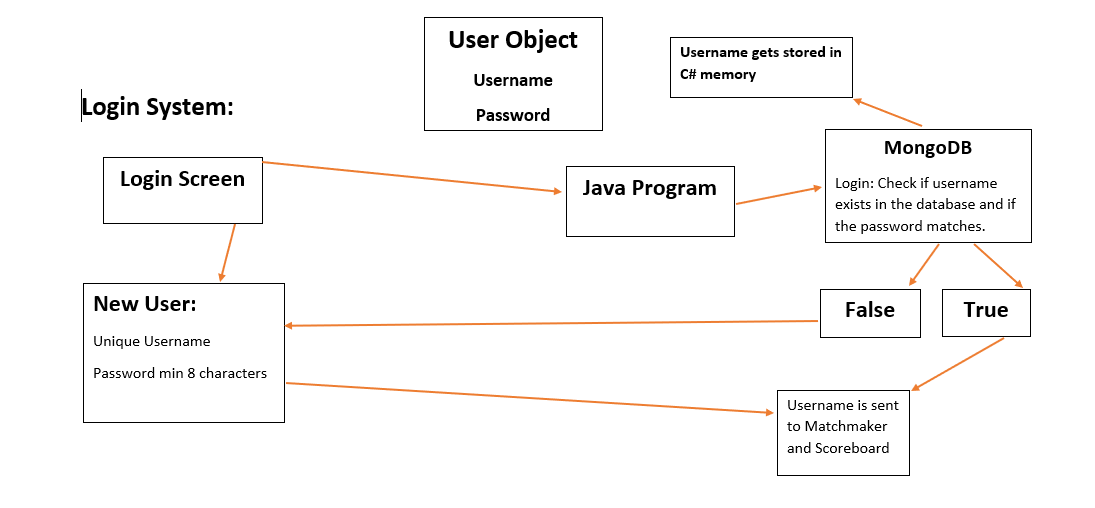
\includegraphics[width=1\columnwidth]{img/LoginSystem.PNG}
Overview of Log-in System

\subsection {Match Maker}\newline
Our match making system
The match making system allows users the option to either host a game or find a game to join. Hosting a game means the user is hosting a game on his own network/machine. Joining a game simply allows you to join a game that is being hosted by someone else.\newline

The user name that has been stored in memory in C\# is sent to the match maker. If the user chooses to host a game his username and IP address is sent to the redis database. The username and IP address is then stored in a struct and added to a list of users who want to host a game. The username is then sent back to the match maker screen and a join button appears next to his name. Once other users decide to join the game the users are redirected to the game lobby screen and wait for all users interested in playing, for a limited amount of time, to join and then are brought to play the game.\newline

If the user decides he does not want to host a game he clicks on the find game button which sends a request to the redis database that sends back a list of users who are hosting a game. The user then clicks the join button next to the hosts name. The user then gets redirected to the game lobby where he waits for others to join the game then he is brought to play the game. 
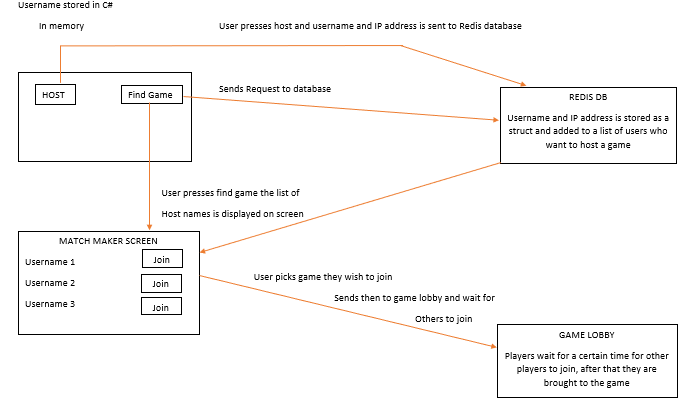
\includegraphics[width=1\columnwidth]{img/redisMatch.PNG}

Overview of Match Maker System
\subsection {Score Board}

\newline

The scoreboard will be the last window the user will interact with. Once the race has ended, the game sends a list of the player objects containing the player username and the points the player received for their position in the race. Once the list is received, a loop runs through the objects and the player name and points received are printed to screen using GUI text field in Unity.
\newline

Next the program will serialize the list as XML for the purpose of sending to the MariaDB database running on the Virtual machine. Before this is done the object must be tagged with the Serializable attribute. It then creates an XML document and declaration and a loop sends the object to the XML file. (The file is not actual created; the XML is saved to a variable). This is done using the XMLSerializer class.
\cite {93513120150101}
\bibliographystyle{plain}
\newline

The program then makes use of the TCP Client class in C\#. The program makes a connection to a socket listening on the virtual machine. Once the connection is made the variable containing the XML is passed to a byte array which is sent using the Network Stream class. This is done by reading the data in and using the write method in the Network Stream class.
\cite {27494020090101}
\bibliographystyle{plain}
\newline

The python program on the virtual machine then receives the XML as a byte stream it decodes the bytes, then it converts them to string and using ElementTree converts them back into XML. It then passes the XML into a second python file called ScoreboardDB. There it takes the XML passed from the Client Connection file and passes UserName & Score in to two lists one called playerNames and the other called playerScore.
\newline

The program then connects to the MariaDB and runs a query to either add the player if they don't already exist or to update there score if they do exist. This is wrapped in a try/catch to bring up an error if for any reason the data cant be added to the database or if a connection the database can't be made.
\newline

After the database has been updated with the latest results the rankDB method is called and it assigns the players rank to a list called playerRank. There rank is based on there total score from all races to writeToXML  definition it adds the results to an XML file which is not an actual file but a BytesIO stream used so to add the XML header which can't be added in python with creating a file or a binary file stream as used here. This is then passed back to the ClientConnection file. Then on the same connection that the XML was received the updated XML is returned to the C# program.    
\newline

The next step in the program is to receive the updated XML using the StreamReader class, making use of the TCP getSteam method available in C#. This data is then read in and saved as XML file in order to deserialize back to an object. This is done by again using the XMLSerializer class, but this time using deserialise method. The file is opened using the FileStream class and a loop runs over the XML and deserialises the file back into a list of objects. This new and updated list is then rendered to screen using GUI text field in Unity.
\newline

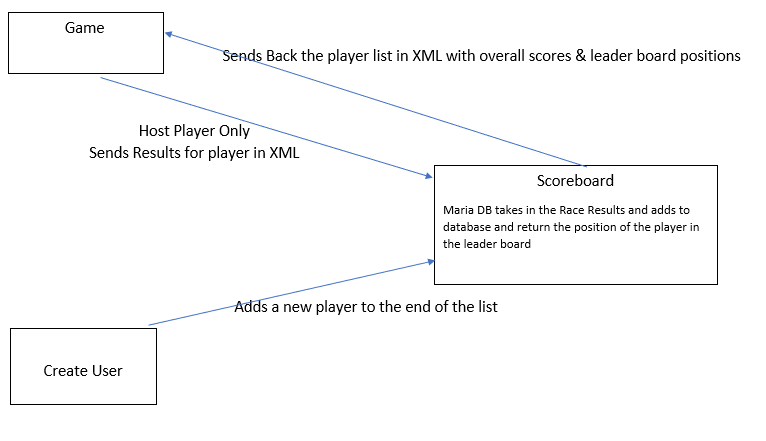
\includegraphics[width=1\columnwidth]{img/scoreBoard.PNG}

Overview of Score Board System

\newpage
\section{Implementation}


\subsection{Game Engine}
Our first decision was to choose a game engine to design the game with. As we had some previous experience with Unity through other modules of our course, and we all had the software installed on our personal computers, it was an easy decision. As Unity works with the C# language, it was much better for us as we all had the necessary software and editor already installed.  
\subsection{Virtual Machine}
The process of choosing a cloud-based platform involved researching what was available to us for free. We explored using a google cloud platform machine but we choose to use AWS. We choose to deploy an AWS virtual machine using a windows 10 operating system. We all had previous experience working with an AWS virtual machine through other modules in our course and setting up the machine was quite painless. We also had previous experience working with sockets to make connections on an AWS machine from a previous module. For ease of access we uploaded the AWS.rdp file to our shared github repository. This allowed us to connect to the machine while working together and individually.\newline

Working with AWS can sometimes be difficult as it only allows one user to access the machine at any given time. This resulted in the creation of a messaging group between all group members which was used to collaborate, and delegate time spent on the virtual machine.\newline
\cite{13214346620180901}
\bibliographystyle{plain}
\newline
Installed on the Virtual Machine
\begin{itemize}
\item MongoDB, RedisDB, MariaDB
\item Eclipse Oxygen IDE
\item Visual Studio Code IDE
\item Docker
\item Heidi
\item Go Lang compiler
\item Python compiler
\end{itemize}

\subsection{Databases}
\subsubsection{Log-in Database}
The choice and implementation of the data bases took a bit longer to finish. We decided to use several database in order to display the heterogeneous aspect of the project. As the project made use of several data bases, we had to make sure we had the right one for each section of the project. For the log-in system we had first decided to use a MongoDB Atlas database. This is a cloud-based version of MongoDB. It had all the same capabilities of the original but is hosted on a cloud-based service of your choice.
\newline

This was not a good choice for us as we would have been charged for the service, and as we would be been testing and sending data so often, we could see ourselves breaking the free threshold. With this in mind, we decided to go with MongoDB community edition as it was an open source release. We would also have full control of the data base and be able to turn it off and make changes whenever we had to. We also had some experience using MongoDB for a previous module.
\newline

To install MongoDB:
\begin{itemize}
\item Click on the file just downloaded which opens the installer.
\item Click Next.
\item Accept Terms and Conditions and click Next.
\item Choose Complete Setup.
\item Click Install.
\item Click Finish.
\end{itemize}
\newline

To setup MongoDB:
\begin{itemize}
\item Open the Windows cmd prompt and navigate to the following folder:
\item C: Program Files MongoDB Server 4.0.3 bin 
\item Start the mongo daemon as follows:
\item Mongod
\item In a new Windows cmd prompt  navigate to the bin folder:
\item C: Program Files MongoDB Server 4.0.3 bin
\item Start mongoDB by entering this command:
\item	mongo
\end{itemize}
\newline
\subsubsection{Match Maker Database}
For our match making system we needed a data base that would work well with the Go programming language. We first looked at using a CouchDB. This proved a bit difficult to implement with Go. We had the data base set up but were unable to get the program to sent data to it. Also, with CouchDB working with a file-based system we did not think it was a good fit.
\newline

We then tested using a RedisDB for our purposes. This database was a better fit for us, as it was an open sourced and made use of in memory data storage. It was also very easy to implement using Go.
\newline

To install RedisDB:
\begin{itemize}
\item Download the .tar file installation package
\item CD to the .tar file location 
\item Open a cmd prompt window and run the command
\item  tar vxf < tarfile name >
\item Then run the command 
\item sudo ./install.sh -s /var/run/redislabs
\end{itemize}
\newline
\subsubsection{Score Board Database}
For the scoreboard database, we originally looked at using a NEO4J database.
The reason for this was because we were using Python to connect to the database, and we had heard that NEO4J worked well with it. After installing and testing it, we found it was not a viable option for us. NEO4J is a graph database management system and was not appropriate for our needs.
We next looked at using a MariaDB for the scoreboard. This is an SQL relation database and was a much better option for the scoreboard.
\newline

As we were using MariaDB, we decided to install HeidiSQl on the virtual machine. This is a tool that allows a user to create and query a database using a user interface, rather than write the SQL commands from scratch. As this would be a time saving advantage, we installed it on the virtual machine.
\newline

To install MariaDB:
\begin{itemize}
\item Click on the downloaded file.
\item The MariaDB setup wizard will launch, click next.
\item Accept the License Agreement and click next.
\item Here you can set your Root password and select to allow to access the database from remote machines.
\item Click next on the default instance properties 
\item Click install 
\end{itemize}
\newline

To install HeidiSQL:
\begin{itemize}
\item Run HeidiSQL
\item Click the new button in session manager
\item Select Network type MySql (TCP/IP)
\item Set Hostname as 127.0.0.1
\item Set User as root from MariaDB setup 
\item Set Password as password from MariaDB setup 
\item Set Port to 5004 (or any available port)
\item Then click open
\end{itemize}
\newpage
\subsection{XML/JSON}
For the project, we could have easily used one of these for the sending of information throughout the system. Since this was a learning experience, we decided to use both of these mediums in order to gain a better understanding and working knowledge of them. 
\section{Integration and System Testing}


We were going to use Loadview system to test the scalability of the project but with the version of aws that we were using we could not perform testing on it with out going over the free tier limit, as on occasion we were already going over the free tier limit. \newline 
We have tested on multiple devices that we can send and receive data from each of the databases as needed throughout the game. \newline

\subsection{Integration Testing } \newline

\subsubsection{Username Validation} \newline
When the user enters their username to create a new user if they enter a name that already being used, they are prompted to try again. They won’t be allowed to use a username that isn’t unique.  \newline
\textbf{Result: Pass} 

\subsubsection{Password Validation}  \newline
The password must be at least eight characters long or the user is prompted to renter  there password and is not allowed to proceed until the password is entered as required.\newline
\textbf{Result: Pass}

\subsubsection{Login Validation}  \newline
When the user attempts to login with their username and password, it is sent to the MongoDB as a user object. The database is then searched to confirm that the user exists and that they entered the correct password for that username. If they enter incorrect information they are shown an error that says invalid log in details. They then have the option to click okay and they will be brought back to the login screen and can enter the correct information or create a new user account.\newline 
\textbf{Result: Pass}

\subsubsection{Host Validation}\newline
When a user decides to host a game. There name and IP address are sent to the Redis DB and added to a list of hosts that is displayed whenever a user wants to join a game. When a user tries to join a game, they should receive an up to date list of hosts that have opted to host a game.\newline
\textbf{Result: Pass}

\subsubsection{User can Respawn}\newline
When racing if the user goes off the track. They can press the R key (Desktop) and they will be respawned back onto the track near where they went off. \newline 
\textbf{Result: Pass}

\subsubsection{User can Jump}\newline
At any point in the race the user can press space bar in desktop and ? in VR and there vehicle will make a slight jump. \newline 
\textbf{Result: Pass}

\subsubsection{Controls testing desktop}\newline
Users will be able to control the cart using their keyboard keys W, A, S & D. W key will control going forward. A key will control turning leaf. D key will cover turning right. S key will cover going in reverse. \newline
\textbf{Result: Partial Pass}: Going forward, turning left and turning right all worked as expected. Reversing was unresponsive. 

\subsubsection{Scoreboard Race End}\newline
After the race is completed the results are sent from the C\# program to the MariaDB on the AWS. The database is updated with the results from the race and the updated rankings are sent back to the host. The host then displays the results for the rest of the users to see.\newline 
\textbf{Result: Pass}

\subsubsection{Scoreboard New User}\newline
After the race is completed the results are sent from the C# program to the MariaDB on the AWS. If there is a new user there record is created and there score is set to the results from that race. The updated rankings are then returned to the host to display.\newline
\textbf{Result: Pass}

\subsubsection{Scoreboard displays only the users who raced}\newline

\subsubsection{Scoreboard displays updated world rankings}\newline


\subsection{System Testing } \newline

